\documentclass[11pt,a4paper]{article}

\usepackage[T1]{fontenc}
\usepackage{lmodern}
\usepackage{microtype}
\usepackage[margin=1in,headheight=24pt]{geometry}
\usepackage[table]{xcolor}
\usepackage{graphicx}
\usepackage{tabularx}
\usepackage{array}
\makeatletter
\@ifundefined{insert@pcolumn}{\let\insert@pcolumn\insert@column}{}
\makeatother
\usepackage{longtable}
\usepackage{enumitem}
\usepackage{titlesec}
\usepackage{fancyhdr}
\usepackage{caption}
\usepackage{float}
\usepackage{listings}
\usepackage{multicol}
\usepackage{tikz}
\usetikzlibrary{calc}
\usepackage[hidelinks]{hyperref}

\definecolor{Ink}{HTML}{1F2933}
\definecolor{MutedInk}{HTML}{5F6C7B}
\definecolor{DeepTeal}{HTML}{2E6F73}
\definecolor{DustyBlue}{HTML}{8AA8BD}
\definecolor{SoftMint}{HTML}{DDEFE8}
\definecolor{PowderBlue}{HTML}{E8F1F6}
\definecolor{Blush}{HTML}{F1D9D4}
\definecolor{WarmSand}{HTML}{F6F1E8}
\definecolor{Lavender}{HTML}{ECE7F5}
\definecolor{HeaderGray}{HTML}{6FA8AA}
\definecolor{RowGray}{HTML}{F4F6F8}
\definecolor{CodeBg}{HTML}{F8FAFB}
\definecolor{CodeRule}{HTML}{C8D7DF}
\definecolor{CodeAccent}{HTML}{B77765}
\definecolor{PageHeaderGray}{HTML}{A5ADB6}
\definecolor{NodeCity}{HTML}{65DFAF}
\definecolor{NodeCompany}{HTML}{FFBFB5}
\definecolor{NodeCourse}{HTML}{EA8FF6}
\definecolor{NodeDepartment}{HTML}{80BABC}
\definecolor{NodeEnrollment}{HTML}{79F5D6}
\definecolor{NodeEvent}{HTML}{B5E6FE}
\definecolor{NodeEventRegistration}{HTML}{56C4CA}
\definecolor{NodeGovernmentProject}{HTML}{F4A4D1}
\definecolor{NodeHospital}{HTML}{FFACCE}
\definecolor{NodeMinistry}{HTML}{9AC098}
\definecolor{NodePatient}{HTML}{C5AA7B}
\definecolor{NodeProperty}{HTML}{FF8D69}
\definecolor{NodeStudent}{HTML}{D7C3F4}
\definecolor{NodeUniversity}{HTML}{E4ABBE}

\hypersetup{
  pdftitle={Neo4j Graph Database Implementation for KRG Open Data},
  pdfauthor={Sawab Hussein, Mohammed Salah, Asmaa Salih},
  pdfsubject={Advanced Database Systems Group Project},
  pdfkeywords={Neo4j, Cypher, graph database, KRG, open data}
}

\graphicspath{{figures/}{./}}
\setlength{\parindent}{0pt}
\setlength{\parskip}{0.62em}
\renewcommand{\arraystretch}{1.10}
\setlist[itemize]{leftmargin=1.5em,itemsep=0.25em,topsep=0.25em}
\setlist[enumerate]{leftmargin=1.5em,itemsep=0.25em,topsep=0.25em}

\pagestyle{fancy}
\fancyhf{}
\lhead{\textcolor{PageHeaderGray}{\itshape Neo4j KRG Graph Report}}
\rhead{\textcolor{PageHeaderGray}{\itshape Advanced Database Systems}}
\cfoot{\textcolor{MutedInk}{\thepage}}
\renewcommand{\headrulewidth}{0pt}
\renewcommand{\headrule}{\hbox to\headwidth{\color{CodeRule}\leaders\hrule height \headrulewidth\hfill}}

\titleformat{\section}
  {\normalfont\LARGE\bfseries\color{DeepTeal}}
  {\thesection}
  {0.65em}
  {}
\titleformat{\subsection}
  {\normalfont\large\bfseries\color{Ink}}
  {\thesubsection}
  {0.65em}
  {}
\titlespacing*{\section}{0pt}{1.4em}{0.5em}
\titlespacing*{\subsection}{0pt}{0.9em}{0.25em}

\captionsetup{
  font=small,
  labelfont={bf,color=DeepTeal},
  textfont={color=MutedInk},
  justification=centering,
  singlelinecheck=false
}

\newcolumntype{Y}{>{\raggedright\arraybackslash}X}
\newcolumntype{Z}{>{\centering\arraybackslash}X}
\newcommand{\thcell}[1]{\hfil\mbox{\rule[-0.45ex]{0pt}{2.8ex}\textcolor{white}{\scriptsize\bfseries #1}}\hfil\null}
\newenvironment{softtabularx}[1]{%
  \begingroup\footnotesize
  \rowcolors{2}{RowGray}{white}%
  \tabularx{\linewidth}{#1}%
}{%
  \endtabularx%
  \rowcolors{2}{}{}%
  \endgroup
}
\newcommand{\taskmeta}[3]{%
  \begin{softtabularx}{>{\bfseries\color{Ink}}m{0.27\linewidth}Y}
    \rowcolor{HeaderGray}
    \thcell{Item} & \thcell{Details} \\
    Question & #1 \\
    Graph shape & #2 \\
    Visualization purpose & #3 \\
  \end{softtabularx}
}
\newcommand{\resultfigure}[3]{%
  \begin{figure}[H]
    \centering
    \includegraphics[width=0.86\linewidth,height=#2\textheight,keepaspectratio]{#1}
    \caption{#3}
  \end{figure}
}
\newcommand{\pairedresultfigures}[3]{%
  \begin{figure}[H]
    \centering
    \begin{minipage}[t]{0.46\linewidth}
      \centering
      \includegraphics[width=\linewidth,height=0.24\textheight,keepaspectratio]{#1}\\[-0.2em]
      {\small\color{MutedInk}LIMIT 30}
    \end{minipage}\hfill
    \begin{minipage}[t]{0.46\linewidth}
      \centering
      \includegraphics[width=\linewidth,height=0.24\textheight,keepaspectratio]{#2}\\[-0.2em]
      {\small\color{MutedInk}LIMIT 1000}
    \end{minipage}
    \caption{#3}
  \end{figure}
}
\newcommand{\legendnode}[2]{%
  \tikz[baseline=-0.6ex]\fill[#1] (0,0) circle (0.55ex);%
  \hspace{0.22em}{\textcolor{#1}{\scriptsize\bfseries #2}}%
}
\newcommand{\nodelegend}[1]{%
  \begin{center}
    \begin{minipage}{0.88\linewidth}
      \centering
      \setlength{\spaceskip}{0.42em}%
      #1
    \end{minipage}
  \end{center}
}

\lstdefinelanguage{Cypher}{
  morekeywords={
    MATCH,OPTIONAL,RETURN,WHERE,WITH,ORDER,BY,DESC,ASC,LIMIT,LOAD,CSV,WITH,HEADERS,
    FROM,AS,MERGE,SET,CREATE,INDEX,IF,NOT,EXISTS,FOR,ON,CALL,IN,TRANSACTIONS,OF,ROWS,
    DISTINCT,COUNT,CASE,WHEN,THEN,ELSE,END,IS,NULL,collect,toInteger,toFloat
  },
  sensitive=false,
  morecomment=[l]{//},
  morestring=[b]'
}

\lstdefinestyle{cypherstyle}{
  language=Cypher,
  basicstyle=\ttfamily\footnotesize,
  keywordstyle=\color{DeepTeal}\bfseries,
  commentstyle=\color{MutedInk}\itshape,
  stringstyle=\color{CodeAccent},
  numbers=left,
  numberstyle=\tiny\color{MutedInk},
  numbersep=8pt,
  stepnumber=1,
  showstringspaces=false,
  breaklines=true,
  breakatwhitespace=false,
  columns=fullflexible,
  keepspaces=true,
  backgroundcolor=\color{CodeBg},
  frame=single,
  rulecolor=\color{CodeRule},
  framerule=0.4pt,
  framesep=6pt,
  xleftmargin=0.25em,
  xrightmargin=0.25em,
  tabsize=2
}
\lstdefinestyle{appendixcode}{
  style=cypherstyle,
  basicstyle=\ttfamily\fontsize{5.2}{5.8}\selectfont,
  numberstyle=\fontsize{4.8}{5.2}\selectfont\color{MutedInk},
  numbersep=4pt,
  framesep=3pt,
  framerule=0.3pt,
  xleftmargin=0pt,
  xrightmargin=0pt,
  aboveskip=0.85em,
  belowskip=1.15em,
  captionpos=t
}
\lstset{style=cypherstyle}
\newenvironment{compactappendixcode}{%
  \begingroup
  \setlength{\columnsep}{1.15cm}
  \setlength{\columnseprule}{0pt}
  \captionsetup[lstlisting]{font=scriptsize,skip=4pt}
  \lstset{style=appendixcode}
  \begin{multicols}{2}
  \raggedcolumns
}{%
  \end{multicols}
  \lstset{style=cypherstyle}
  \endgroup
}

\begin{document}
\hypersetup{pageanchor=false}

\begin{titlepage}
  \thispagestyle{empty}
  \centering
  \vspace*{0.25cm}

  
\includegraphics[width=0.30\textwidth]{AUK-logo.png}

  \vspace{0.45cm}
  {\large\color{Ink}\bfseries American University of Kurdistan, Duhok\par}
  \vspace{0.12cm}
  {\normalsize\color{DeepTeal}MSc in Artificial Intelligence\par}
  {\normalsize\color{MutedInk}Advanced Database Systems -- 101\par}

  \vspace{0.45cm}
  {\color{DeepTeal}\rule{0.72\textwidth}{1.1pt}\par}
  \vspace{0.35cm}
  {\fontsize{25}{30}\selectfont\bfseries\color{Ink}
  Neo4j Graph Database\\Implementation for KRG\\Open Data\par}
  \vspace{0.32cm}
  {\large\color{MutedInk}
  Graph modeling, data loading, relationship design, and visual Cypher analysis\par}
  \vspace{0.38cm}
  {\color{DeepTeal}\rule{0.72\textwidth}{1.1pt}\par}

  \vspace{0.58cm}
  {\large\color{Ink}\bfseries Team Members\par}
  \vspace{0.14cm}
  {\large\color{MutedInk}Sawab Hussein \quad Mohammed Salah \quad Asmaa Salih\par}

  \vspace{0.42cm}
  {\color{Ink}\bfseries Instructor:\ }{\color{MutedInk}Dr. Shamal AL-Dohuki\par}
  {\color{Ink}\bfseries DBMS:\ }{\color{MutedInk}Neo4j\par}
  {\color{Ink}\bfseries Date:\ }{\color{MutedInk}April 2026\par}
\end{titlepage}

\hypersetup{pageanchor=true}
\pagenumbering{roman}
\tableofcontents
\clearpage

\pagenumbering{arabic}

\section{Project Context}

\subsection{Dataset Scope}

The project uses thirteen CSV tables, each containing 1,000 records. The tables cover five major domains: education, healthcare, government, business and property, and events.

\begin{softtabularx}{>{\bfseries\color{Ink}}m{0.26\linewidth}m{0.15\linewidth}Y}
  \rowcolor{HeaderGray}
  \thcell{Domain} & \thcell{Tables} & \thcell{Main entities} \\
  Education & 5 & Universities, departments, courses, students, enrollments \\
  Healthcare & 2 & Hospitals and patients \\
  Government & 2 & Ministries and government projects \\
  Business and property & 2 & Companies and real estate properties \\
  Events & 2 & Events and event registrations \\
\end{softtabularx}

\subsection{Neo4j Analytical Capabilities}

Neo4j can be used to follow paths, compare connected neighborhoods, find hubs, expose cross-city movement, and combine multiple domains in one traversal. In this report, those capabilities are used to analyze student mobility, healthcare referrals, ministry control, event concentration, city stress, and public-investment pressure. The graph model is powerful for analysis because relationships are stored as first-class structure, so a question can move naturally from one entity to another instead of being rebuilt as a temporary table join.

The complete Cypher used to create indexes, load nodes, build relationships, verify the city hub, and run the ten visual tasks is included in the appendix.

\section{Data Fetching and Graph Construction}

\subsection{Preparation and Import Method}

The data was loaded from CSV files placed inside the Neo4j import directory. The workflow used \texttt{LOAD CSV WITH HEADERS} so each row could be mapped into a node or relationship using named columns. This approach is repeatable, transparent, and easy to audit because the Cypher scripts show exactly which CSV field becomes which graph property.

Before importing relationships, the project created indexes for the entity identifiers used in joins. This is an important performance step because relationship creation repeatedly matches existing nodes by IDs such as \texttt{student\_id}, \texttt{course\_id}, \texttt{hospital\_id}, and \texttt{city.name}.
\subsection{Node Loading Strategy}

Nodes were loaded with \texttt{MERGE} instead of \texttt{CREATE}. This makes the import idempotent: running the same load block again updates the existing node rather than duplicating it. Properties were converted into typed values where useful, including integers for counts and years, and floating-point values for revenue, budget, and prices.
This pattern was repeated across companies, students, universities, courses, departments, hospitals, patients, events, ministries, government projects, properties, enrollments, and event registrations.

\subsection{The City Hub Design}

The clever modeling action in this project is the creation of \texttt{City} as a shared hub. Instead of letting every table keep city as a disconnected string value, the import process gathers city names from all relevant CSV files and merges them into a small set of city nodes.
This is unique and important in Neo4j because the city is no longer passive metadata. It becomes an active connector in the graph. From the same city node, Neo4j can traverse to hospitals, events, projects, companies, universities, properties, students, and patients. The model turns geography into an analytical backbone.

\subsection{Relationship Creation}

Relationships were created after the nodes existed. This separation keeps the import process reliable: first build the entities, then connect them. For larger CSV files, relationship creation used transaction batching through \texttt{IN TRANSACTIONS OF 500 ROWS}, which reduces memory pressure and supports efficient bulk loading.

The relationship layer captures both structural relationships and contextual movement. For example, \texttt{LIVES\_IN} records a person's home city, while \texttt{LOCATED\_IN} records where an institution, event, property, or project exists. Comparing those paths is what reveals cross-city student mobility and healthcare movement.

\subsection{Verification Queries}

After importing, the graph can be checked through count queries. The node verification query confirms the expected labels, while the relationship verification query confirms the volume of each edge type.

The city hub can be verified with a single query that groups every entity type connected to a city:
\section{Graph Schema}

\subsection{Node Labels}

\begin{softtabularx}{>{\bfseries\color{Ink}}m{0.28\linewidth}Y}
  \rowcolor{HeaderGray}
  \thcell{Node label} & \thcell{Role in the graph} \\
  City & Geographic hub shared across all major domains \\
  Student & Education actor with home city and university path \\
  University & Higher education institution connected to departments and city \\
  Department & Academic unit inside a university \\
  Course & Course connected to departments and students \\
  Enrollment & Source record for student-course participation \\
  Hospital & Healthcare institution connected to patients and city \\
  Patient & Healthcare actor with home city and admission path \\
  Ministry & Public administration body managing projects \\
  GovernmentProject & Public investment project connected to ministries and cities \\
  Company & Business entity located in a city \\
  Property & Real estate asset located in a city \\
  Event & Event activity located in a city \\
  EventRegistration & Registration record connected to events \\
\end{softtabularx}

\subsection{Relationship Model}

\begin{softtabularx}{>{\ttfamily\footnotesize\color{Ink}}m{0.55\linewidth}Y}
  \rowcolor{HeaderGray}
  \thcell{Relationship} & \thcell{Meaning} \\
  (:University)-[:LOCATED\_IN]->(:City) & Places universities in the city hub model \\
  (:Hospital)-[:LOCATED\_IN]->(:City) & Places hospitals in the city hub model \\
  (:Company)-[:LOCATED\_IN]->(:City) & Connects business activity to geography \\
  (:Event)-[:LOCATED\_IN]->(:City) & Connects events to host cities \\
  (:Property)-[:LOCATED\_IN]->(:City) & Connects real estate supply to cities \\
  (:GovernmentProject)-[:LOCATED\_IN]->(:City) & Connects public projects to implementation cities \\
  (:Ministry)-[:LOCATED\_IN]->(:City) & Locates administrative bodies \\
  (:Student)-[:LIVES\_IN]->(:City) & Records student home cities \\
  (:Student)-[:STUDIES\_AT]->(:University) & Connects students to universities \\
  (:Student)-[:ENROLLED\_IN]->(:Course) & Captures academic enrollment relationships \\
  (:Course)-[:BELONGS\_TO]->(:Department) & Locates courses inside departments \\
  (:Department)-[:PART\_OF]->(:University) & Connects departments to universities \\
  (:Patient)-[:LIVES\_IN]->(:City) & Records patient home cities \\
  (:Patient)-[:ADMITTED\_TO]->(:Hospital) & Captures healthcare admission relationships \\
  (:GovernmentProject)-[:MANAGED\_BY]->(:Ministry) & Connects projects to administrative ownership \\
  (:EventRegistration)-[:REGISTERED\_FOR]->(:Event) & Connects registrations to event participation \\
\end{softtabularx}

\subsection{Design Benefit}

The schema supports both direct entity lookup and multi-hop analytical paths. For example, a ministry can be connected to a project, the project can be connected to a city, and the same city can be connected to high-priced properties. The graph therefore supports mixed administrative and economic questions without first flattening the data into one table.

\section{Visual Cypher Task Portfolio}

The following ten tasks are based on \texttt{10\_Neo4j\_Visual\_Tasks.md}. Each task includes its analytical question, graph shape, Neo4j Browser result image, Cypher query, and interpretation. Where both screenshots are available, the report places the LIMIT 30 and LIMIT 1000 results side by side so the reader can compare readable samples with denser graph output.

\subsection{Task 1: City as a Central Multi-Sector Hub}

\taskmeta
  {Which city acts as the strongest shared hub across education, healthcare, business, events, and real estate?}
  {\texttt{University / Hospital / Company / Event / Property --[:LOCATED\_IN]--> City}}
  {Shows the city as the central integration point across independent sectors.}

\pairedresultfigures{task01_city_hub.png}{task01_city_hub_1000.png}{Task 1 Neo4j graph result comparison: city as a multi-sector hub.}
\nodelegend{
  \legendnode{NodeCity}{City}
  \legendnode{NodeUniversity}{University}
  \legendnode{NodeHospital}{Hospital}
  \legendnode{NodeCompany}{Company}
  \legendnode{NodeEvent}{Event}
  \legendnode{NodeProperty}{Property}
}
This is the foundation query for the report. It proves that \texttt{City} is not just a property but a navigable graph hub connecting five sectors through one consistent relationship pattern.

\subsection{Task 2: Patient and Hospital Movement}

\taskmeta
  {How do patients move from their home city to the hospital system, and are they treated locally or outside their city?}
  {\texttt{Patient --[:LIVES\_IN]--> HomeCity} and \texttt{Patient --[:ADMITTED\_TO]--> Hospital --[:LOCATED\_IN]--> HospitalCity}}
  {Separates residence from treatment location so local and cross-city healthcare patterns become visible.}

\pairedresultfigures{task02_patient_hospital.png}{task02_patient_hospital_1000.png}{Task 2 Neo4j graph result comparison: patient residence and hospital treatment paths.}
\nodelegend{
  \legendnode{NodePatient}{Patient}
  \legendnode{NodeCity}{City}
  \legendnode{NodeHospital}{Hospital}
}
The query illustrates why graph paths are expressive for healthcare analysis. One patient can be read as a bridge between a home city and a hospital city, and the \texttt{CASE} expression labels the path as local or cross-city treatment.

\subsection{Task 3: Government Project Network}

\taskmeta
  {Which ministries control public projects, and how are those projects distributed across cities?}
  {\texttt{Ministry <--[:MANAGED\_BY]-- GovernmentProject --[:LOCATED\_IN]--> City}}
  {Places each project between administrative ownership and geographic implementation.}

\pairedresultfigures{task03_government_projects.png}{task03_government_projects_1000.png}{Task 3 Neo4j graph result comparison: ministries, government projects, and cities.}
\nodelegend{
  \legendnode{NodeGovernmentProject}{GovernmentProject}
  \legendnode{NodeMinistry}{Ministry}
  \legendnode{NodeCity}{City}
}
This graph makes public administration easier to inspect. Projects are not isolated budget records; they sit between a ministry and a city, enabling questions about distribution, responsibility, and public service reach.

\subsection{Task 4: Cross-City Student Mobility}

\taskmeta
  {Which students leave their home city for university, and which cities are sending or receiving students?}
  {\texttt{Student --[:LIVES\_IN]--> HomeCity} and \texttt{Student --[:STUDIES\_AT]--> University --[:LOCATED\_IN]--> UniversityCity}}
  {Shows students as bridge nodes between origin cities and university cities.}

\resultfigure{task04_student_mobility.png}{0.36}{Task 4 Neo4j graph result: cross-city student mobility, LIMIT 1000.}
\nodelegend{
  \legendnode{NodeStudent}{Student}
  \legendnode{NodeCity}{City}
  \legendnode{NodeUniversity}{University}
}
The \texttt{WHERE} clause filters the graph to the most interesting cases: students whose study location differs from their home city. This turns a simple enrollment dataset into a mobility network.

\subsection{Task 5: Full Academic Path for Students}

\taskmeta
  {How does each student connect into the full academic structure of courses, departments, universities, and locations?}
  {\texttt{Student --[:ENROLLED\_IN]--> Course --[:BELONGS\_TO]--> Department --[:PART\_OF]--> University --[:LOCATED\_IN]--> City}}
  {Presents the complete academic chain from individual learner to city.}

\pairedresultfigures{task05_academic_path.png}{task05_academic_path_1000.png}{Task 5 Neo4j graph result comparison: complete academic path.}
\nodelegend{
  \legendnode{NodeStudent}{Student}
  \legendnode{NodeCourse}{Course}
  \legendnode{NodeDepartment}{Department}
  \legendnode{NodeUniversity}{University}
  \legendnode{NodeCity}{City}
}
This is the most complete education query in the portfolio. It demonstrates a layered graph path where a student connects to curriculum, department, institution, and city in a single traversal.

\subsection{Task 6: Event Registrations and Their Cities}

\taskmeta
  {How do registrations connect to events, and how are events distributed across cities?}
  {\texttt{EventRegistration --[:REGISTERED\_FOR]--> Event --[:LOCATED\_IN]--> City}}
  {Shows event popularity and geographic grouping through registration clusters.}

\pairedresultfigures{task06_event_registrations.png}{task06_event_registrations_1000.png}{Task 6 Neo4j graph result comparison: event registrations and city grouping.}
\nodelegend{
  \legendnode{NodeEventRegistration}{EventRegistration}
  \legendnode{NodeEvent}{Event}
  \legendnode{NodeCity}{City}
}
The event graph connects individual registration records to hosted events and then to the city hub. Dense registration clusters reveal event concentration, while the city link makes geographic comparison possible.

\subsection{Task 7: Cross-City Healthcare Referral Network}

\taskmeta
  {Which cities depend on hospitals in other cities, and where is cross-city healthcare movement strongest?}
  {\texttt{Patient --[:LIVES\_IN]--> HomeCity} and \texttt{Patient --[:ADMITTED\_TO]--> Hospital --[:LOCATED\_IN]--> HospitalCity}}
  {Highlights referral-like movement by comparing patient residence and hospital location.}

\pairedresultfigures{task07_healthcare_referral.png}{task07_healthcare_referral_1000.png}{Task 7 Neo4j graph result comparison: cross-city healthcare referral network.}
\nodelegend{
  \legendnode{NodePatient}{Patient}
  \legendnode{NodeCity}{City}
  \legendnode{NodeHospital}{Hospital}
}
This query extends Task 2 by emphasizing referral classification. It is useful for identifying where healthcare demand crosses city boundaries and which hospital cities may be absorbing outside patients.

\subsection{Task 8: Ministry Cross-City Project Control}

\taskmeta
  {Is public project management local, or are some cities controlled administratively from other cities?}
  {\texttt{Ministry --[:LOCATED\_IN]--> MinistryCity}, \texttt{GovernmentProject --[:MANAGED\_BY]--> Ministry}, and \texttt{GovernmentProject --[:LOCATED\_IN]--> ProjectCity}}
  {Reveals administrative centralization by comparing ministry city and project city.}

\pairedresultfigures{task08_ministry_control.png}{task08_ministry_control_1000.png}{Task 8 Neo4j graph result comparison: cross-city ministry project control.}
\nodelegend{
  \legendnode{NodeMinistry}{Ministry}
  \legendnode{NodeCity}{City}
  \legendnode{NodeGovernmentProject}{GovernmentProject}
}
The city hub makes this query especially concise. The graph compares two city paths around the same project: the ministry's city and the project's city. Cross-city matches point to centralized administrative control.

\subsection{Task 9: City Stress Index Graph}

\taskmeta
  {Which cities carry the highest multi-sector load across healthcare, events, government projects, and real estate?}
  {\texttt{Patient / Event / GovernmentProject / Property --> City}, ranked by combined \texttt{StressScore}}
  {Uses the city hub to compute a multi-sector load index and then visualize the highest-density city neighborhoods.}

\begin{figure}[H]
  \centering
  \begin{minipage}[c][0.30\textheight][c]{0.46\linewidth}
    \centering
    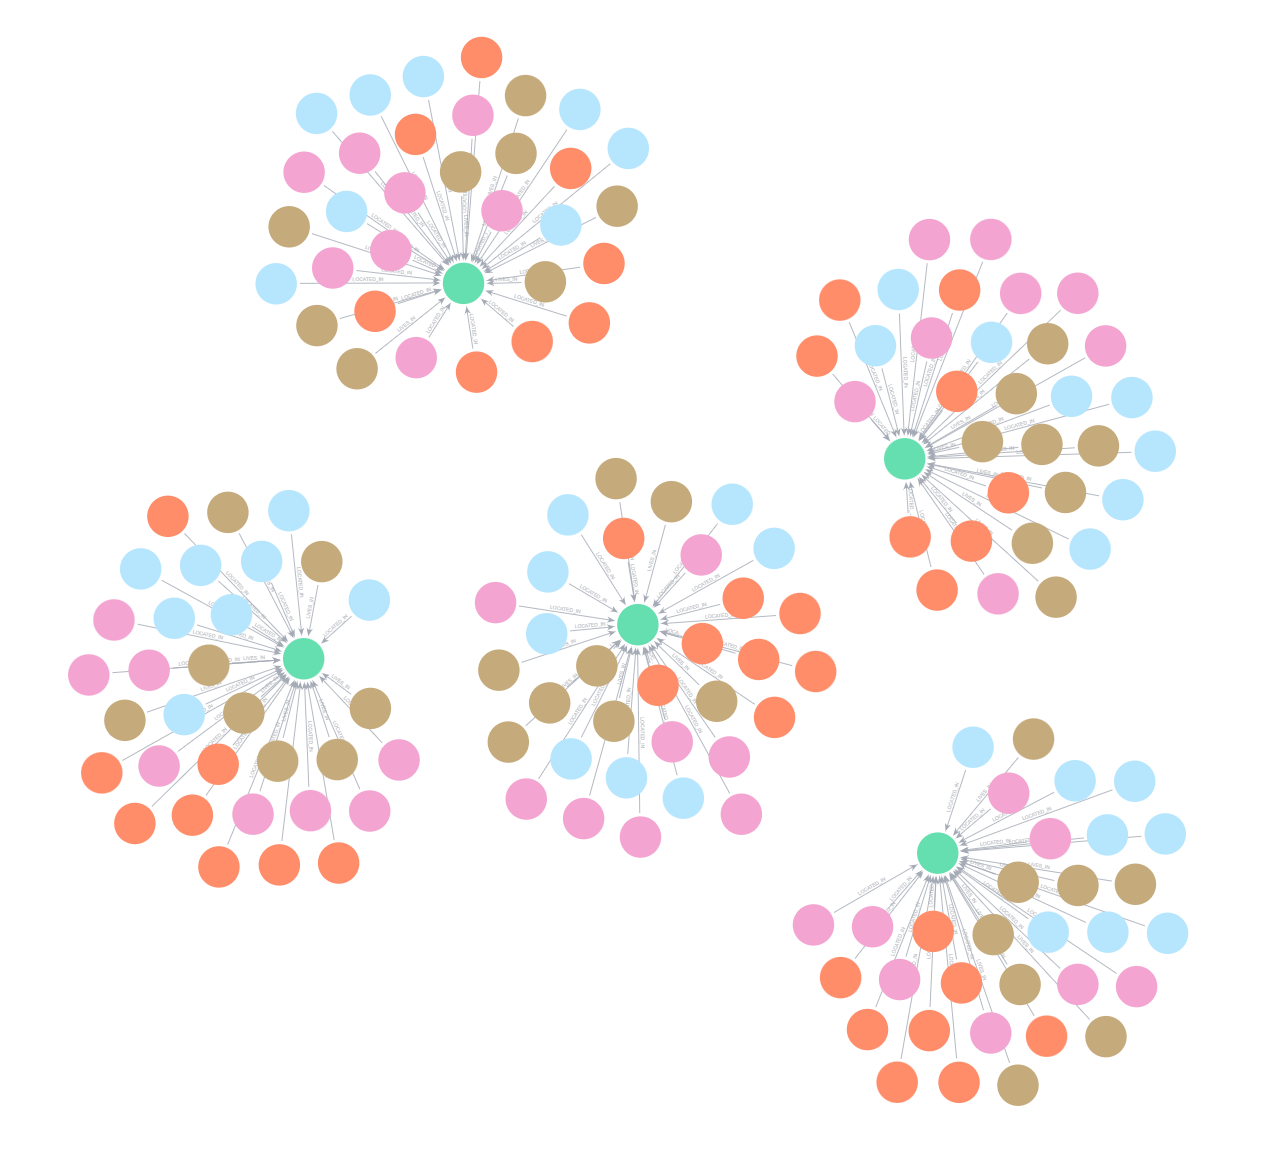
\includegraphics[width=\linewidth,height=0.25\textheight,keepaspectratio]{task09_city_stress.png}\\[-0.2em]
    {\small\color{MutedInk}Graph result}
  \end{minipage}\hfill
  \begin{minipage}[c][0.30\textheight][c]{0.45\linewidth}
    \centering
    {\rowcolors{2}{RowGray}{white}
    \resizebox{\linewidth}{!}{%
    \begin{tabular}{lccccc}
      \rowcolor{HeaderGray}
      \thcell{City} & \thcell{Patients} & \thcell{Events} & \thcell{Projects} & \thcell{Properties} & \thcell{StressScore} \\
      Sulaymaniyah & 198 & 195 & 225 & 202 & 820 \\
      Halabja & 207 & 187 & 197 & 226 & 817 \\
      Duhok & 203 & 223 & 175 & 194 & 795 \\
      Zakho & 200 & 187 & 208 & 198 & 793 \\
      Erbil & 192 & 208 & 195 & 180 & 775 \\
    \end{tabular}}%
    \rowcolors{2}{}{}}
    {\small\color{MutedInk}CSV result table}
  \end{minipage}
  \caption{Task 9 Neo4j result: city stress graph alongside the extracted CSV table.}
\end{figure}
\nodelegend{
  \legendnode{NodeCity}{City}
  \legendnode{NodePatient}{Patient}
  \legendnode{NodeEvent}{Event}
  \legendnode{NodeGovernmentProject}{GovernmentProject}
  \legendnode{NodeProperty}{Property}
}
Task 9 demonstrates analytical use of the city hub. Instead of inspecting one sector at a time, the query computes a combined load using patients, events, projects, and properties. Sulaymaniyah ranks highest in the extracted result, closely followed by Halabja.

\subsection{Task 10: Public Investment and Property Market Pressure}

\taskmeta
  {Which cities show both large public investment and high property prices, suggesting economic pressure or development concentration?}
  {\texttt{Ministry -- GovernmentProject -- City -- Property}}
  {Connects government spending with real estate price signals through the city hub.}

\pairedresultfigures{task10_public_investment.png}{task10_public_investment_1000.png}{Task 10 Neo4j graph result comparison: public investment and property market pressure.}
\nodelegend{
  \legendnode{NodeMinistry}{Ministry}
  \legendnode{NodeGovernmentProject}{GovernmentProject}
  \legendnode{NodeCity}{City}
  \legendnode{NodeProperty}{Property}
}
The final task combines public-sector and property-market data. The city node acts as the bridge between government projects and real estate, enabling analysis of cities where major public spending and expensive properties appear together.

\section{Conclusion}

The project shows how a graph database can turn a multi-table dataset into a connected analytical model. The most important design decision was promoting \texttt{City} into a central node label. That action gives the graph a natural hub that links education, healthcare, government, business, events, and property records.

The implementation also follows sound data engineering practice: identifiers are indexed before relationship creation, nodes are loaded idempotently with \texttt{MERGE}, numeric values are typed during import, and relationship loading is batched for efficiency. The result is a graph that is both visually understandable and analytically useful.

Across the ten visual tasks, Neo4j proves useful not merely as a storage system but as a reasoning interface. It can show mobility, referrals, administrative reach, multi-sector stress, and investment pressure as paths. This path-first view is the central advantage of Neo4j for the KRG open data project.

\appendix
\clearpage
\section{Complete Source Code Appendix}
The following listings reproduce every fenced code block from the two Markdown source files. The main report refers to these blocks rather than repeating the full scripts in the body.

\subsection{fetching\_data.md}
\begin{compactappendixcode}
\lstinputlisting[caption={fetching\_data.md code block 1}]{appendix_code/fetching_data_01.cypher}
\lstinputlisting[caption={fetching\_data.md code block 2}]{appendix_code/fetching_data_02.cypher}
\lstinputlisting[caption={fetching\_data.md code block 3}]{appendix_code/fetching_data_03.cypher}
\lstinputlisting[caption={fetching\_data.md code block 4}]{appendix_code/fetching_data_04.cypher}
\lstinputlisting[caption={fetching\_data.md code block 5}]{appendix_code/fetching_data_05.cypher}
\lstinputlisting[caption={fetching\_data.md code block 6}]{appendix_code/fetching_data_06.cypher}
\lstinputlisting[caption={fetching\_data.md code block 7}]{appendix_code/fetching_data_07.cypher}
\lstinputlisting[caption={fetching\_data.md code block 8}]{appendix_code/fetching_data_08.cypher}
\lstinputlisting[caption={fetching\_data.md code block 9}]{appendix_code/fetching_data_09.cypher}
\lstinputlisting[caption={fetching\_data.md code block 10}]{appendix_code/fetching_data_10.cypher}
\lstinputlisting[caption={fetching\_data.md code block 11}]{appendix_code/fetching_data_11.cypher}
\lstinputlisting[caption={fetching\_data.md code block 12}]{appendix_code/fetching_data_12.cypher}
\lstinputlisting[caption={fetching\_data.md code block 13}]{appendix_code/fetching_data_13.cypher}
\lstinputlisting[caption={fetching\_data.md code block 14}]{appendix_code/fetching_data_14.cypher}
\lstinputlisting[caption={fetching\_data.md code block 15}]{appendix_code/fetching_data_15.cypher}
\lstinputlisting[caption={fetching\_data.md code block 16}]{appendix_code/fetching_data_16.cypher}
\lstinputlisting[caption={fetching\_data.md code block 17}]{appendix_code/fetching_data_17.cypher}
\lstinputlisting[caption={fetching\_data.md code block 18}]{appendix_code/fetching_data_18.cypher}
\lstinputlisting[caption={fetching\_data.md code block 19}]{appendix_code/fetching_data_19.cypher}
\lstinputlisting[caption={fetching\_data.md code block 20}]{appendix_code/fetching_data_20.cypher}
\lstinputlisting[caption={fetching\_data.md code block 21}]{appendix_code/fetching_data_21.cypher}
\lstinputlisting[caption={fetching\_data.md code block 22}]{appendix_code/fetching_data_22.cypher}
\lstinputlisting[caption={fetching\_data.md code block 23}]{appendix_code/fetching_data_23.cypher}
\lstinputlisting[caption={fetching\_data.md code block 24}]{appendix_code/fetching_data_24.cypher}
\lstinputlisting[caption={fetching\_data.md code block 25}]{appendix_code/fetching_data_25.cypher}
\lstinputlisting[caption={fetching\_data.md code block 26}]{appendix_code/fetching_data_26.cypher}
\lstinputlisting[caption={fetching\_data.md code block 27}]{appendix_code/fetching_data_27.cypher}
\lstinputlisting[caption={fetching\_data.md code block 28}]{appendix_code/fetching_data_28.cypher}
\lstinputlisting[caption={fetching\_data.md code block 29}]{appendix_code/fetching_data_29.cypher}
\lstinputlisting[caption={fetching\_data.md code block 30}]{appendix_code/fetching_data_30.cypher}
\lstinputlisting[caption={fetching\_data.md code block 31}]{appendix_code/fetching_data_31.cypher}
\lstinputlisting[caption={fetching\_data.md code block 32}]{appendix_code/fetching_data_32.cypher}
\lstinputlisting[caption={fetching\_data.md code block 33}]{appendix_code/fetching_data_33.cypher}
\lstinputlisting[caption={fetching\_data.md code block 34}]{appendix_code/fetching_data_34.cypher}
\lstinputlisting[caption={fetching\_data.md code block 35}]{appendix_code/fetching_data_35.cypher}
\lstinputlisting[caption={fetching\_data.md code block 36}]{appendix_code/fetching_data_36.cypher}
\lstinputlisting[caption={fetching\_data.md code block 37}]{appendix_code/fetching_data_37.cypher}
\lstinputlisting[caption={fetching\_data.md code block 38}]{appendix_code/fetching_data_38.cypher}
\end{compactappendixcode}

\subsection{10\_Neo4j\_Visual\_Tasks.md}
\begin{compactappendixcode}
\lstinputlisting[caption={10\_Neo4j\_Visual\_Tasks.md code block 1}]{appendix_code/visual_tasks_01.cypher}
\lstinputlisting[caption={10\_Neo4j\_Visual\_Tasks.md code block 2}]{appendix_code/visual_tasks_02.cypher}
\lstinputlisting[caption={10\_Neo4j\_Visual\_Tasks.md code block 3}]{appendix_code/visual_tasks_03.cypher}
\lstinputlisting[caption={10\_Neo4j\_Visual\_Tasks.md code block 4}]{appendix_code/visual_tasks_04.cypher}
\lstinputlisting[caption={10\_Neo4j\_Visual\_Tasks.md code block 5}]{appendix_code/visual_tasks_05.cypher}
\lstinputlisting[caption={10\_Neo4j\_Visual\_Tasks.md code block 6}]{appendix_code/visual_tasks_06.cypher}
\lstinputlisting[caption={10\_Neo4j\_Visual\_Tasks.md code block 7}]{appendix_code/visual_tasks_07.cypher}
\lstinputlisting[caption={10\_Neo4j\_Visual\_Tasks.md code block 8}]{appendix_code/visual_tasks_08.cypher}
\lstinputlisting[caption={10\_Neo4j\_Visual\_Tasks.md code block 9}]{appendix_code/visual_tasks_09.cypher}
\lstinputlisting[caption={10\_Neo4j\_Visual\_Tasks.md code block 10}]{appendix_code/visual_tasks_10.cypher}
\lstinputlisting[caption={10\_Neo4j\_Visual\_Tasks.md code block 11}]{appendix_code/visual_tasks_11.cypher}
\lstinputlisting[caption={10\_Neo4j\_Visual\_Tasks.md code block 13}]{appendix_code/visual_tasks_13.txt}
\end{compactappendixcode}


\end{document}

